
%% bare_jrnl.tex
%% V1.4b
%% 2015/08/26
%% by Michael Shell
%% see http://www.michaelshell.org/
%% for current contact information.
%%
%% This is a skeleton file demonstrating the use of IEEEtran.cls
%% (requires IEEEtran.cls version 1.8b or later) with an IEEE
%% journal paper.
%%
%% Support sites:
%% http://www.michaelshell.org/tex/ieeetran/
%% http://www.ctan.org/pkg/ieeetran
%% and
%% http://www.ieee.org/

%%*************************************************************************
%% Legal Notice:
%% This code is offered as-is without any warranty either expressed or
%% implied; without even the implied warranty of MERCHANTABILITY or
%% FITNESS FOR A PARTICULAR PURPOSE!
%% User assumes all risk.
%% In no event shall the IEEE or any contributor to this code be liable for
%% any damages or losses, including, but not limited to, incidental,
%% consequential, or any other damages, resulting from the use or misuse
%% of any information contained here.
%%
%% All comments are the opinions of their respective authors and are not
%% necessarily endorsed by the IEEE.
%%
%% This work is distributed under the LaTeX Project Public License (LPPL)
%% ( http://www.latex-project.org/ ) version 1.3, and may be freely used,
%% distributed and modified. A copy of the LPPL, version 1.3, is included
%% in the base LaTeX documentation of all distributions of LaTeX released
%% 2003/12/01 or later.
%% Retain all contribution notices and credits.
%% ** Modified files should be clearly indicated as such, including  **
%% ** renaming them and changing author support contact information. **
%%*************************************************************************


% *** Authors should verify (and, if needed, correct) their LaTeX system  ***
% *** with the testflow diagnostic prior to trusting their LaTeX platform ***
% *** with production work. The IEEE's font choices and paper sizes can   ***
% *** trigger bugs that do not appear when using other class files.       ***                          ***
% The testflow support page is at:
% http://www.michaelshell.org/tex/testflow/



\documentclass[lettersize,journal]{IEEEtran}
%
% If IEEEtran.cls has not been installed into the LaTeX system files,
% manually specify the path to it like:
% \documentclass[journal]{../sty/IEEEtran}





% Some very useful LaTeX packages include:
% (uncomment the ones you want to load)


% *** MISC UTILITY PACKAGES ***
%
%\usepackage{ifpdf}
% Heiko Oberdiek's ifpdf.sty is very useful if you need conditional
% compilation based on whether the output is pdf or dvi.
% usage:
% \ifpdf
%   % pdf code
% \else
%   % dvi code
% \fi
% The latest version of ifpdf.sty can be obtained from:
% http://www.ctan.org/pkg/ifpdf
% Also, note that IEEEtran.cls V1.7 and later provides a builtin
% \ifCLASSINFOpdf conditional that works the same way.
% When switching from latex to pdflatex and vice-versa, the compiler may
% have to be run twice to clear warning/error messages.






% *** CITATION PACKAGES ***
%
\usepackage{cite}
% cite.sty was written by Donald Arseneau
% V1.6 and later of IEEEtran pre-defines the format of the cite.sty package
% \cite{} output to follow that of the IEEE. Loading the cite package will
% result in citation numbers being automatically sorted and properly
% "compressed/ranged". e.g., [1], [9], [2], [7], [5], [6] without using
% cite.sty will become [1], [2], [5]--[7], [9] using cite.sty. cite.sty's
% \cite will automatically add leading space, if needed. Use cite.sty's
% noadjust option (cite.sty V3.8 and later) if you want to turn this off
% such as if a citation ever needs to be enclosed in parenthesis.
% cite.sty is already installed on most LaTeX systems. Be sure and use
% version 5.0 (2009-03-20) and later if using hyperref.sty.
% The latest version can be obtained at:
% http://www.ctan.org/pkg/cite
% The documentation is contained in the cite.sty file itself.






% *** GRAPHICS RELATED PACKAGES ***
%
\usepackage[pdftex]{graphicx}
\ifCLASSINFOpdf
  % \usepackage[pdftex]{graphicx}
  % declare the path(s) where your graphic files are
  % \graphicspath{{../pdf/}{../jpeg/}}
  % and their extensions so you won't have to specify these with
  % every instance of \includegraphics
  % \DeclareGraphicsExtensions{.pdf,.jpeg,.png}
\else
  % or other class option (dvipsone, dvipdf, if not using dvips). graphicx
  % will default to the driver specified in the system graphics.cfg if no
  % driver is specified.
  % \usepackage[dvips]{graphicx}
  % declare the path(s) where your graphic files are
  % \graphicspath{{../eps/}}
  % and their extensions so you won't have to specify these with
  % every instance of \includegraphics
  % \DeclareGraphicsExtensions{.eps}
\fi
% graphicx was written by David Carlisle and Sebastian Rahtz. It is
% required if you want graphics, photos, etc. graphicx.sty is already
% installed on most LaTeX systems. The latest version and documentation
% can be obtained at:
% http://www.ctan.org/pkg/graphicx
% Another good source of documentation is "Using Imported Graphics in
% LaTeX2e" by Keith Reckdahl which can be found at:
% http://www.ctan.org/pkg/epslatex
%
% latex, and pdflatex in dvi mode, support graphics in encapsulated
% postscript (.eps) format. pdflatex in pdf mode supports graphics
% in .pdf, .jpeg, .png and .mps (metapost) formats. Users should ensure
% that all non-photo figures use a vector format (.eps, .pdf, .mps) and
% not a bitmapped formats (.jpeg, .png). The IEEE frowns on bitmapped formats
% which can result in "jaggedy"/blurry rendering of lines and letters as
% well as large increases in file sizes.
%
% You can find documentation about the pdfTeX application at:
% http://www.tug.org/applications/pdftex





% *** MATH PACKAGES ***
%
\usepackage{amsmath,amssymb}
% A popular package from the American Mathematical Society that provides
% many useful and powerful commands for dealing with mathematics.
%
% Note that the amsmath package sets \interdisplaylinepenalty to 10000
% thus preventing page breaks from occurring within multiline equations. Use:
%\interdisplaylinepenalty=2500
% after loading amsmath to restore such page breaks as IEEEtran.cls normally
% does. amsmath.sty is already installed on most LaTeX systems. The latest
% version and documentation can be obtained at:
% http://www.ctan.org/pkg/amsmath





% *** SPECIALIZED LIST PACKAGES ***
%
%\usepackage{algorithmic}
% algorithmic.sty was written by Peter Williams and Rogerio Brito.
% This package provides an algorithmic environment fo describing algorithms.
% You can use the algorithmic environment in-text or within a figure
% environment to provide for a floating algorithm. Do NOT use the algorithm
% floating environment provided by algorithm.sty (by the same authors) or
% algorithm2e.sty (by Christophe Fiorio) as the IEEE does not use dedicated
% algorithm float types and packages that provide these will not provide
% correct IEEE style captions. The latest version and documentation of
% algorithmic.sty can be obtained at:
% http://www.ctan.org/pkg/algorithms
% Also of interest may be the (relatively newer and more customizable)
% algorithmicx.sty package by Szasz Janos:
% http://www.ctan.org/pkg/algorithmicx




% *** ALIGNMENT PACKAGES ***
%
%\usepackage{array}
% Frank Mittelbach's and David Carlisle's array.sty patches and improves
% the standard LaTeX2e array and tabular environments to provide better
% appearance and additional user controls. As the default LaTeX2e table
% generation code is lacking to the point of almost being broken with
% respect to the quality of the end results, all users are strongly
% advised to use an enhanced (at the very least that provided by array.sty)
% set of table tools. array.sty is already installed on most systems. The
% latest version and documentation can be obtained at:
% http://www.ctan.org/pkg/array


% IEEEtran contains the IEEEeqnarray family of commands that can be used to
% generate multiline equations as well as matrices, tables, etc., of high
% quality.




% *** SUBFIGURE PACKAGES ***
\ifCLASSOPTIONcompsoc
 \usepackage[caption=false,font=normalsize,labelfont=sf,textfont=sf]{subfig}
\else
 \usepackage[caption=false,font=footnotesize]{subfig}
\fi
% subfig.sty, written by Steven Douglas Cochran, is the modern replacement
% for subfigure.sty, the latter of which is no longer maintained and is
% incompatible with some LaTeX packages including fixltx2e. However,
% subfig.sty requires and automatically loads Axel Sommerfeldt's caption.sty
% which will override IEEEtran.cls' handling of captions and this will result
% in non-IEEE style figure/table captions. To prevent this problem, be sure
% and invoke subfig.sty's "caption=false" package option (available since
% subfig.sty version 1.3, 2005/06/28) as this is will preserve IEEEtran.cls
% handling of captions.
% Note that the Computer Society format requires a larger sans serif font
% than the serif footnote size font used in traditional IEEE formatting
% and thus the need to invoke different subfig.sty package options depending
% on whether compsoc mode has been enabled.
%
% The latest version and documentation of subfig.sty can be obtained at:
% http://www.ctan.org/pkg/subfig




% *** FLOAT PACKAGES ***
%
%\usepackage{fixltx2e}
% fixltx2e, the successor to the earlier fix2col.sty, was written by
% Frank Mittelbach and David Carlisle. This package corrects a few problems
% in the LaTeX2e kernel, the most notable of which is that in current
% LaTeX2e releases, the ordering of single and double column floats is not
% guaranteed to be preserved. Thus, an unpatched LaTeX2e can allow a
% single column figure to be placed prior to an earlier double column
% figure.
% Be aware that LaTeX2e kernels dated 2015 and later have fixltx2e.sty's
% corrections already built into the system in which case a warning will
% be issued if an attempt is made to load fixltx2e.sty as it is no longer
% needed.
% The latest version and documentation can be found at:
% http://www.ctan.org/pkg/fixltx2e


%\usepackage{stfloats}
% stfloats.sty was written by Sigitas Tolusis. This package gives LaTeX2e
% the ability to do double column floats at the bottom of the page as well
% as the top. (e.g., "\begin{figure*}[!b]" is not normally possible in
% LaTeX2e). It also provides a command:
%\fnbelowfloat
% to enable the placement of footnotes below bottom floats (the standard
% LaTeX2e kernel puts them above bottom floats). This is an invasive package
% which rewrites many portions of the LaTeX2e float routines. It may not work
% with other packages that modify the LaTeX2e float routines. The latest
% version and documentation can be obtained at:
% http://www.ctan.org/pkg/stfloats
% Do not use the stfloats baselinefloat ability as the IEEE does not allow
% \baselineskip to stretch. Authors submitting work to the IEEE should note
% that the IEEE rarely uses double column equations and that authors should try
% to avoid such use. Do not be tempted to use the cuted.sty or midfloat.sty
% packages (also by Sigitas Tolusis) as the IEEE does not format its papers in
% such ways.
% Do not attempt to use stfloats with fixltx2e as they are incompatible.
% Instead, use Morten Hogholm'a dblfloatfix which combines the features
% of both fixltx2e and stfloats:
%
% \usepackage{dblfloatfix}
% The latest version can be found at:
% http://www.ctan.org/pkg/dblfloatfix




%\ifCLASSOPTIONcaptionsoff
%  \usepackage[nomarkers]{endfloat}
% \let\MYoriglatexcaption\caption
% \renewcommand{\caption}[2][\relax]{\MYoriglatexcaption[#2]{#2}}
%\fi
% endfloat.sty was written by James Darrell McCauley, Jeff Goldberg and
% Axel Sommerfeldt. This package may be useful when used in conjunction with
% IEEEtran.cls'  captionsoff option. Some IEEE journals/societies require that
% submissions have lists of figures/tables at the end of the paper and that
% figures/tables without any captions are placed on a page by themselves at
% the end of the document. If needed, the draftcls IEEEtran class option or
% \CLASSINPUTbaselinestretch interface can be used to increase the line
% spacing as well. Be sure and use the nomarkers option of endfloat to
% prevent endfloat from "marking" where the figures would have been placed
% in the text. The two hack lines of code above are a slight modification of
% that suggested by in the endfloat docs (section 8.4.1) to ensure that
% the full captions always appear in the list of figures/tables - even if
% the user used the short optional argument of \caption[]{}.
% IEEE papers do not typically make use of \caption[]'s optional argument,
% so this should not be an issue. A similar trick can be used to disable
% captions of packages such as subfig.sty that lack options to turn off
% the subcaptions:
% For subfig.sty:
% \let\MYorigsubfloat\subfloat
% \renewcommand{\subfloat}[2][\relax]{\MYorigsubfloat[]{#2}}
% However, the above trick will not work if both optional arguments of
% the \subfloat command are used. Furthermore, there needs to be a
% description of each subfigure *somewhere* and endfloat does not add
% subfigure captions to its list of figures. Thus, the best approach is to
% avoid the use of subfigure captions (many IEEE journals avoid them anyway)
% and instead reference/explain all the subfigures within the main caption.
% The latest version of endfloat.sty and its documentation can obtained at:
% http://www.ctan.org/pkg/endfloat
%
% The IEEEtran \ifCLASSOPTIONcaptionsoff conditional can also be used
% later in the document, say, to conditionally put the References on a
% page by themselves.




% *** PDF, URL AND HYPERLINK PACKAGES ***
%
\usepackage{url}
% url.sty was written by Donald Arseneau. It provides better support for
% handling and breaking URLs. url.sty is already installed on most LaTeX
% systems. The latest version and documentation can be obtained at:
% http://www.ctan.org/pkg/url
% Basically, \url{my_url_here}.




% *** Do not adjust lengths that control margins, column widths, etc. ***
% *** Do not use packages that alter fonts (such as pslatex).         ***
% There should be no need to do such things with IEEEtran.cls V1.6 and later.
% (Unless specifically asked to do so by the journal or conference you plan
% to submit to, of course. )

\usepackage{booktabs}
\usepackage{url,xcolor}

% correct bad hyphenation here
\hyphenation{op-tical net-works semi-conduc-tor}


\def\permille{\ensuremath{{}^\text{o}\mkern-5mu/\mkern-3mu_\text{oo}}}
\newcommand{\interval}[2]{\mathopen{[}#1\,;#2\mathclose{]}}

\begin{document}
%
% paper title
% Titles are generally capitalized except for words such as a, an, and, as,
% at, but, by, for, in, nor, of, on, or, the, to and up, which are usually
% not capitalized unless they are the first or last word of the title.
% Linebreaks \\ can be used within to get better formatting as desired.
% Do not put math or special symbols in the title.
\title{Joint self-supervised blind denoising and noise estimation}
%
%
% author names and IEEE memberships
% note positions of commas and nonbreaking spaces ( ~ ) LaTeX will not break
% a structure at a ~ so this keeps an author's name from being broken across
% two lines.
% use \thanks{} to gain access to the first footnote area
% a separate \thanks must be used for each paragraph as LaTeX2e's \thanks
% was not built to handle multiple paragraphs
%

\author{Jean Ollion\thanks{Jean Ollion: SABILab, France.}, Charles Ollion\thanks{Charles Ollion:  CMAP, Ecole Polytechnique, Institut Polytechnique de Paris, France.},  \'Elisabeth Gassiat\thanks{\'Elisabeth Gassiat: Universit\'e Paris-Saclay, CNRS, Laboratoire de math\'ematiques d'Orsay, 91405, Orsay, France.},   Luc Leh\'ericy\thanks{Luc Leh\'ericy:   Laboratoire J. A. Dieudonn\'e, Universit\'e C\^ote d'Azur, CNRS, 06108, Nice, France.} and~Sylvain Le Corff\thanks{Sylvain Le Corff: Samovar, T\'el\'ecom SudParis, D\'epartement CITI, Institut Polyechnique de Paris, France.}}
%        and~Jane~Doe,~\IEEEmembership{Life~Fellow,~IEEE}% <-this % stops a space
%\thanks{M. Shell was with the Department
%of Electrical and Computer Engineering, Georgia Institute of Technology, Atlanta,
%GA, 30332 USA e-mail: (see http://www.michaelshell.org/contact.html).}% <-this % stops a space
%\thanks{J. Doe and J. Doe are with Anonymous University.}% <-this % stops a space
%\thanks{Manuscript received April 19, 2005; revised August 26, 2015.}}

% note the % following the last \IEEEmembership and also \thanks -
% these prevent an unwanted space from occurring between the last author name
% and the end of the author line. i.e., if you had this:
%
% \author{....lastname \thanks{...} \thanks{...} }
%                     ^------------^------------^----Do not want these spaces!
%
% a space would be appended to the last name and could cause every name on that
% line to be shifted left slightly. This is one of those "LaTeX things". For
% instance, "\textbf{A} \textbf{B}" will typeset as "A B" not "AB". To get
% "AB" then you have to do: "\textbf{A}\textbf{B}"
% \thanks is no different in this regard, so shield the last } of each \thanks
% that ends a line with a % and do not let a space in before the next \thanks.
% Spaces after \IEEEmembership other than the last one are OK (and needed) as
% you are supposed to have spaces between the names. For what it is worth,
% this is a minor point as most people would not even notice if the said evil
% space somehow managed to creep in.



% The paper headers
%\markboth{Journal of \LaTeX\ Class Files,~Vol.~14, No.~8, August~2015}%
%{Shell \MakeLowercase{\textit{et al.}}: Bare Demo of IEEEtran.cls for IEEE Journals}

% The only time the second header will appear is for the odd numbered pages
% after the title page when using the twoside option.
%
% *** Note that you probably will NOT want to include the author's ***
% *** name in the headers of peer review papers.                   ***
% You can use \ifCLASSOPTIONpeerreview for conditional compilation here if
% you desire.




% If you want to put a publisher's ID mark on the page you can do it like
% this:
%\IEEEpubid{0000--0000/00\$00.00~\copyright~2015 IEEE}
% Remember, if you use this you must call \IEEEpubidadjcol in the second
% column for its text to clear the IEEEpubid mark.



% use for special paper notices
%\IEEEspecialpapernotice{(Invited Paper)}




% make the title area
\maketitle

% As a general rule, do not put math, special symbols or citations
% in the abstract or keywords.
\begin{abstract}
We propose a novel self-supervised image blind denoising approach in which two neural networks jointly predict the clean signal and infer the noise distribution.
Assuming that the noisy observations are independent conditionally to the signal, the networks can be trained jointly without any clean data. This approach is particularly relevant for biomedical image denoising where the noise is difficult to model precisely and clean training data are usually unavailable. Our method significantly outperforms current state-of-the-art self-supervised blind denoising algorithms on six publicly available biomedical image datasets, as well as its supervised counterpart. We also show empirically that it is able to capture noise distributions efficiently, both on different synthetic noise models and real multimodal and skewed data.
Finally, the described framework is simple, lightweight and computationally efficient, making it useful in practical cases.
\end{abstract}

% Note that keywords are not normally used for peerreview papers.
\begin{IEEEkeywords}
Blind denoising, Self-supervised learning.
\end{IEEEkeywords}






% For peer review papers, you can put extra information on the cover
% page as needed:
% \ifCLASSOPTIONpeerreview
% \begin{center} \bfseries EDICS Category: 3-BBND \end{center}
% \fi
%
% For peerreview papers, this IEEEtran command inserts a page break and
% creates the second title. It will be ignored for other modes.
\IEEEpeerreviewmaketitle


\section{Introduction}
\label{sec:introduction}

Image denoising is a well-known Computer Vision task designed to restore pictures taken in poor imaging conditions. In scientific imagery (microscopy, astronomy, etc.) for instance,  the optical setting may produce very noisy images, which limits their interpretability or their automatic processing.
Formally, image denoising is the process of recovering a clean signal $X_s$ given an observation $Y_s$ at location $s\in \mathbb{N}^2$ corrupted by an additive noise $\varepsilon_s$. Classical denoising approaches are model-driven in the sense that they rely on strong assumptions on the noise distribution or on the structure of the signal but are often limited by the relevance of these assumptions.
Recently, efficient data-driven methods have emerged. Most of them assume that pairs made of noisy data $Y_s$ associated with a clean signal $X_s$ are available in a supervised learning framework, see for instance \cite{weigert2017content}. In \cite{lehtinen2018noise2noise}, the authors have demonstrated that it is possible to train an efficient denoising method using only pairs of independent noisy measurements $(Y_s^1, Y_s^2)$ of the same signal $X_s$. Such assumptions have also been used to solve deconvolution problems with repeated measurements as in \cite{delaigle2008deconvolution}. However, obtaining independent observations of the same signal is often unrealistic in practice.

Recent self-supervised methods have overcome this limitation \cite{batson2019noise2self,krull2018noise2void,quan2020self} for instance by training a neural network to predict the value of a (corrupted) pixel $Y_s$ only using the noisy observations of the surrounding pixels. In such frameworks, the trained network extracts some local structure in the signal and therefore can be used as a denoiser. Such approaches are referred to as \textit{blind-denoising} as they only assume that the noises associated with different observations are independent and centered.
This is well suited to typical microscopy settings, in which the clean image is unavailable and the noise process is complex and not known.

These methods rely on training a function $f_\theta$ depending on an unknown parameter $\theta$, usually implemented as a convolutional neural network. Using only the noisy observations and a binary mask $M$, the objective is to minimize a self-supervision loss of the form $\theta\mapsto \sum_{i=1}^N \|f_\theta(Y^{masked})_{s_i} - Y_{s_i}\|_2^2$,
where $Y^{masked}$ is an image in which pixels have been masked using $M$. This masking step is crucial to foster learning of local structure in the signal to predict the masked values.

While these methods are appealing in practice and result in efficient denoising functions, they suffer from several drawbacks:
1) it is not well understood why they are so effective in practice, i.e. what type of noise they are able to remove, and how sensible they are to the masking scheme for instance;
2) they often suffer from high frequency denoising artifacts known as \textit{checkerboard pattern}.

To address these issues, we introduce a novel self-supervised method, based on the joint training of two neural networks referred to as D-net (denoiser net) and N-net (noise net). Similar to previous works, the denoiser is a convolutional neural network and receives a masked input during training. The flexible N-net recovers precisely the noise distribution during training, even for complex asymmetric noises.
We derive this method from a different mathematical modeling of the denoising problem, which may open avenues for better understanding of why self-supervised methods achieve remarkable results.

The contribution of this work can be summarized as follows:
\begin{itemize}
\item we introduce a novel self-supervised blind-denoising method, modeling both the signal and the noise distributions;
\item we show that the N-net recovers the noise distribution efficiently in varying experiments with synthetic and real noises;
\item the proposed architectures outperform state-of-the-art algorithms over 6 standard microscopy datasets, without introducing denoising artifacts.
\end{itemize}

\section{Related work}
\label{sec:related}
\paragraph{Masking and J-invariance}
The most typical class of denoising functions is chosen to be comprised of convolutional neural networks (CNNs), which are heavily parameterized functions and are not restricted to solve denoising problems. As an important consequence, a naive self-supervised loss without any masking would result in learning the identity function (i.e. the function outputing the noisy observation $Y_s$ if it is not masked in the input data), as the considered CNNs can typically implement it. Starting from this intuition, many of the related works can be viewed as different masking schemes. This has been described in the \textit{J-invariant} framework introduced by \cite{batson2019noise2self}: a \textit{J-invariant} function does not depend on a few selected dimensions $J$ of its input variables; typically this translates into a convolutional function which does not depend on the central pixel of the convolutional receptive field, but rather on the observations of neighboring pixels\footnote{Those functions excluding the central pixel are sometimes also called \textit{blind spot}, not to be confused with \textit{blind denoising} in which the noise process is not known.}.

The first masked self-supervised denoising methods were introduced by Noise2Void (N2V) \cite{krull2018noise2void}, in which $\{(Y^{masked}_{s_i},Y_{s_i})\}_{1\leqslant i\leqslant N}$ are sampled randomly in the picture, and masking consists in replacing $Y_{s_i}$ by a random observed value in its neighborhood, with a positive probability of replacing $Y_{s_i}$ by itself meaning that leaks in masking are introduced.

Noise2Self (N2S) \cite{batson2019noise2self} masking procedure differs from N2V in the sense that $\{(Y^{masked}_{s_i},Y_{s_i})\}_{1\leqslant i\leqslant N}$ are obtained with a fixed grid, and $Y_i$ is replaced by the average of the 4 direct neighboring observations.
In practice, the masking procedure has a strong impact on training: (i) improving masking schemes can improve denoising performance and (ii) as only masked pixels are used for training, typically representing a few percent of the image, this affects greatly the training efficiency.

The underlying CNN architecture implemented by these works is the U-net \cite{ronneberger2015u}, a typical convolutional autoencoder architecture, involving skip connections, which can reproduce fine grained details, while making use of higher-level spatially coarse information. While showing strong denoising performance in N2S and N2V, they however can produce \textit{checkerboard patterns}, which are high frequency artifacts that arise in the denoised results.
These works have been extended in DecoNoising \cite{goncharova2020} in which a Gaussian convolution is added after the neural network output to simulate microscope Point Spread Function.
This technique improves performances, however the deconvolved image (predicted image before the Gaussian convolution) displays even stronger checkerboard pattern.

It is noteworthy that \cite{broaddus2020removing} showed that when the noise has local correlations (for instance a  directional noise), masking can be adapted to remove them - by masking adjacent pixels in the same direction as the noise spatial correlation for instance.

Finally, a few methods with different have been developed different training schemes, such as Neighbor2Neighbor \cite{huang2021neighbor2neighbor}, in which a pair of sub-sampled images is generated from the noisy image. The author then use this pair in a way similar to \cite{lehtinen2018noise2noise}, in order to train their denoising model with one being the input and the other the output. One of the main benefits is that the whole downsampled image is used for training. On the other hand, it relies heavily on the downsampling procedure and does not enable to learn information about the noise distribution.

\paragraph{J-invariance without masking}
Instead of masking specific pixels, it is possible to design specific convolutional operators to limit the receptive field, ensuring that the resulting function is \textit{J-invariant} by design. This was achieved in \cite{laine2019high} by introducing directional convolution kernels, each kernel has its receptive field restricted to a half-plane that does not contain the central pixel. The associated function then takes values which only depend on pixels in specific directions, ensuring that it does not depend on pixels in the opposite direction. One drawback is that the inference has to be performed four times, one in each direction.

More recently, \cite{lee2020noise2kernel} introduced a combination of specific convolution operators\footnote{It is interesting to note that with standard convolutions, a two layered network already cannot be made independent of the central pixel, which is why the authors had to rely on very specific convolutions.} with dilation and strides, guaranteeing that the function is independent of the central pixel by design, therefore \textit{J-invariant}.

The benefit of these architectures compared to the masking-based training is that all output pixels can contribute to the loss function as in conventional training, rather than just the masked pixels; and they do not require a carefully tuned masking procedure. However, they strongly constrain the network architecture, which can hinder the denoising performance or result in more expensive inference schemes. Moreover, recent work show that fully \textit{J-invariant} models lead to suboptimal performance \cite{xie2020noise2same}.

\paragraph{Contribution of a noise model}
The denoising literature includes few works which explicitly model the noise distribution, either by choosing \textit{a priori} a  family of distributions (e.g. a Gaussian noise), or by selecting a more flexible class of distributions.

The former is illustrated in \cite{laine2019high}, in which three types of corrupting noise are considered: Gaussian noise independent of the signal; Poisson-Gaussian noise, i.e. a Gaussian noise with variance scaling linearly with the signal value; finally impulse noise, i.e. a uniform noise. In each case, the noise parameters are either known or estimated with an auxiliary neural network. As the signal distribution and the noise distribution belong to a known parametric family, the noisy central pixel can be included at test time to improve performances. However, as the noise type has to be chosen \textit{a priori}, the method is restricted to known and synthetic noise types and therefore is a \textit{non-blind denoising} method.

In \cite{krull2019probabilistic,prakash2020fully}, the authors make use of a more flexible noise model, which is a generic modelisation of the conditional distribution of the noise given the signal intensity and thus can better model real noises.
%: $p(y|x) = N(x): \mathbb{R} \to \mathbb{R}$,
In these works, noise models are approximated using 2D histograms of denoised and noisy observed values, either using additional calibration data (in that case the method is not fully self-supervised) or using a previously trained denoising function \cite{prakash2020fully}. This increases the complexity of the method, as it requires several training procedures and calibration.
In the latter variant, the noise distribution is parametrized with a centered Gaussian mixture model with empirically designed constraints.

In \cite{2020DivNoising}, the authors use the Variational Auto\-Encoder formalism, adding a noise model in their architecture.
This provides new interesting possibilities, as it can generate a diversity of denoised results, but sometimes resulting in visual artifacts or blurry results. When co-learning the noise model, the noise variance is an affine function of the signal value, which corresponds to assuming a Poisson-Gaussian noise distribution.

Perhaps closest to our method, in FBI \cite{byun2021fbi}, the authors focus on Poisson-Gaussian noise, enabling to both denoise efficiently and recover the Poisson-Gaussian parameter. However, they rely heavily on their Poisson-Gaussian assumption to derive their image transformation process and loss function, and therefore unadapted to other types of noise. While this assumption is reasonable for some types of real-world noises, it falls short on other cases, typically with Speckle noise, or at extreme values of signal where the noise distribution can be ill-defined.

It is worth noting that supervised \textit{blind denoising} methods have used parametrized noise models, such as \cite{zhang2017beyond,yue2019variational}, which explicitly used large neural networks to model a complex noise, with even less assumptions (it can be slightly structured). Even though the algorithm proposed in \cite{yue2019variational} is able to train jointly a noise network and a denoiser, their modeling only works in a supervised setting.

\paragraph{Chosen approach} Given a short overview of the related denoising, the following summarizes the key differences with our approach:
\begin{itemize}
  \item \textit{J-invariance}: The proposed approach is not strictly \textit{J-invariant}, which enables for more flexibility in the network architectures, as well as the use of the central pixel at test time. This also alleviates the need to have several inferences steps such as in \cite{laine2019high}.
  \item \textit{Modeling the noise}: Our method enables to model and recover the noise distribution. While some other methods also enable this, they rely on a type of noise assumption (typically: Gaussian of Poisson-Gaussian), while our parametrised noise distributions are much more flexible. This is critical in real noise settings where the noise is not standard nor known.
  \item \textit{Joint training}: We propose a single model in which all the parameters of our models are trained joinlty (both the denoising network and the noise model) by optimizing a single criterion. This results in a very simple, practical and stable procedure, which does not require preprocessing or calibration steps.
\end{itemize}

\section{Model}
\label{sec:model}

Estimating a signal corrupted by additive noise is a challenging statistical problem. In such frameworks, the received observation at location $s\in\mathbb{N}^2$, $Y_s$, is given by $Y_s = X_s + \varepsilon_s$,  where $X_s$ is the signal and $\varepsilon_s$ is the noise. A lot of works have been devoted to deconvolution where the aim is to recover the distribution of the signal based on the observations. It has been for instance applied in a large variety of disciplines and has stimulated a great research interest in signal processing \cite{moulines1997maximum,attias1998blind} and in image reconstruction \cite{kundur1996blind,campisi2017blind}, see also  \cite{meister:2009}. Recently, \cite{gassiat:lecorff:lehericy:2021} proved that it is possible to recover the signal distribution when $X$ has at least two dimensions and may be decomposed into two subsets of random variables which satisfy some weak dependency assumption. This identifiability result does not require any assumption on the noise distribution but illustrates that the components of the signal must be dependent to allow its identification. %The results proposed in \cite{gassiat:lecorff:lehericy:2021} motivate the denoising approach introduced in this work where several classes of noises are considered to describe the observations received from the target signal.  %The signal $X$ is modeled as a function of the noisy observation $Y$ and its neighborhood $\Omega_Y$: $X =  \mu_{\theta_p}(\Omega_Y;Y)$.

Let $\mathsf{S}\subset \mathbb{N}^2$ be a finite set corresponding to the pixel location of an image. In this work, for all $s\in\mathsf{S}$, $X_s$ denotes the signal value at location $s$ and $Y_s$ its noisy observation.  For all $s\in \mathsf{S}$, we write %the conditional distribution of $X_s$ given $\{X_u\,;\, u\in \mathsf{S}\,,\, u\neq s\}$ that the observation $Y$ associated with $X$  is given by
%\begin{equation}
%\label{eq:def:Y}
%Y = X + \sigma_{\theta_n}(X)\varepsilon\,,
%\end{equation}
\begin{equation}
\label{eq:def:Y}
Y_s = X_s + \varepsilon_s\,,
\end{equation}
%which means that
%$$
%Y = X + (\mu_{\theta_p}(\Omega_Y;\overline{\Omega_Y})-\mu_{\theta_p}(\Omega_Y;Y)) + \sigma_{\theta_n}(\mu_{\theta_p}(\Omega_Y;\overline{\Omega_Y}))\varepsilon
%$$
%The blind denoising framework introduced in this work can be written as a regression problem where the observations conditionally on $\Omega_Y$ the observation is given by
%$$
%Y = \mu_{\theta_p}(\Omega_Y;\overline{\Omega_Y}) + \sigma_{\theta_n}(\mu_{\theta_p}(\Omega_Y;\overline{\Omega_Y}))\varepsilon\,,
%$$
%where $\varepsilon$ is a centered noise  independent of $X$ and $\sigma^2_{\theta_n}$ is parameterized by a convolutional neural network, called N-net and with unknown weights $\theta_n$.
%This contrasts with most common denoising algorithms where $\varepsilon$ is assumed to be a centered Gaussian random variable and  $x\mapsto \sigma^2_{\theta_n}(x)$ is either known and constant or has a Poisson-Gaussian shape i.e., scales with $\alpha x + \eta^2$.
%As illustrated in Section~\ref{sec:results}, these assumptions do not usually hold, in particular when considering biomedical images, and they may have a severe impact on denoising performances.
where  $(\varepsilon_s)_{s\in \mathsf{S}}$ are signal-dependent random variables. In this paper, we consider the following assumptions.
\begin{itemize}
\item The random variables  $(\varepsilon_s)_{s\in \mathsf{S}}$ are independent conditionally to $(X_s)_{s\in \mathsf{S}}$ and the conditional distribution of $\varepsilon_s$ depends on $X_s$ only.
\item For all $s\in \mathsf{S}$, $\varepsilon_s$ is centered.
\item For all $s\in \mathsf{S}$, conditionally to $X_s $, $\varepsilon_s$ follows a Gaussian mixture model (GMM) with signal-dependent weights $(\alpha_{k,\theta_n}(X_s))_{1\leqslant k\leqslant N}$, means and variances $\{(\mu_{k,\theta_n}(X_s),\sigma_{k,\theta_n}^2(X_s))\}_{1\leqslant k\leqslant N}$.
\end{itemize}
%
%it is assumed that
%%$$
%%\varepsilon \sim \sum_{k=1}^N \alpha_{k,\theta_n}(X)\varphi_{\mu_{k,\theta_n}(X),\sigma_{k,\theta_n}^2(X)}\,,
%%$$
The nonnegative mixture weights $(\alpha_{k,\theta_n}(X_s))_{1\leqslant k\leqslant N}$ are such that $\sum_{k=1}^N\alpha_{k,\theta_n}(X_s) = 1$, and the means and variances $\{(\mu_{k,\theta_n}(X_s),\sigma_{k,\theta_n}^2(X_s))\}_{1\leqslant k\leqslant N}$ of the mixture model are  parameterized by a convolutional neural network, called N-net and with unknown weights $\theta_n$, see Section~\ref{sec:architectures}.


The aim of this paper is to propose an estimator of the signal value without introducing a prior model on $(X_s)_{s\in \mathsf{S}}$. Our approach is motivated by recent data-driven solutions which allow to avoid using too restrictive prior models with poor predictive performance. For all $s\in \mathsf{S}$, let $\Omega_s$ be a neighborhood of $s$, i.e. a set of pixel locations around $s$. In the following, for any finite set $A \subset \mathsf{S}$, $X_A = \{X_s\,;\, s\in A\}$ and $Y_A = \{Y_s\,;\, s\in A\}$. We propose to estimate the conditional mean of $X_s$ given $(Y_s,Y_{\Omega_s})$ by a parametric function denoted by $\mu_{\theta_d}$ so that $\mathbb{E}[X_s|Y_s,Y_{\Omega_s}]$ is estimated by $\mu_{\theta_d}(Y_s,Y_{\Omega_s})$. The function $ \mu_{\theta_d}$ is parameterized by a convolutional neural network, called D-net and with unknown weights $\theta_d$, see Section~\ref{sec:architectures}.

For all $s\in \mathsf{S}$, the conditional likelihood of a the central pixel given its neighborhood is given by
\begin{align*}
p_{\theta}(Y_s|Y_{\Omega_s}) &= \int p_{\theta}(x,Y_s|Y_{\Omega_s}) \mathrm{d}x\,,\\
&= \int p_{\theta}(x|Y_{\Omega_s})p_{\theta}(Y_s|x) \mathrm{d}x\,,
\end{align*}
where the last equality comes from the fact that $Y_s$ is independent of $Y_{\Omega_s}$ given $X_s$. Assuming that $p_{\theta}(\mathrm{d} x_s|Y_{\Omega_s})$ is a peaked distribution, we propose to approximate it by the Dirac mass at $\mu_{\theta_d}(g(Y_{\Omega_s}),Y_{\Omega_s})$, i.e.
$$
p_{\theta}(\mathrm{d} x_s|Y_{\Omega_s})\simeq \delta_{\mu_{\theta_d}(g(Y_{\Omega_s}),Y_{\Omega_s})}(\mathrm{d} x_s)\,,
$$
where $g$ is a known function. In the experiments below, we chose to set $g(Y_{\Omega_s})$ as the empirical mean of the noisy pixels in $Y_{\Omega_s}$.
%which yields the following approximate likelihood:
%$$
%\hat{p}_\theta(Y|\Omega_Y)  = p_{\theta}(Y|\mu_{\theta_d}(\Omega_Y,g(\Omega_Y)))\,.
%$$
%
%
%A natural estimator of $X$ given the noisy observations is $\widehat X = \mu_{\theta_d}(\Omega_Y,Y)$.
%During training this predictor cannot be used to estimate $\theta_d$ and $\theta_n$ as $\mu_{\theta_d}$ would learn to output the noisy observation $Y$ if it is not masked in the input data.
%This is the reason why we adopt a masking approach and assume during training that $\mu_{\theta_d}$ cannot use $Y$ as an input which must be replaced by an estimator.
%In this framework, a genuine prediction of $Y$ is given by $\mathbb{E}[Y|\Omega_Y]$ which we estimate by $\mu_{\theta_d}(\Omega_Y,g(\Omega_Y))$ where $g$ is a known function. %In the experiments below, we chose to set $g(\Omega_Y)$ as the empirical mean of the noisy pixels in $\Omega_Y$.
%In the experiments below, we provide empirical evaluations that choosing $g(\Omega_Y)$ as the empirical mean of the noisy pixels in $\Omega_Y$ is a robust solution while other choices can be made straightforwardly.




%The signal $X$ is then modeled as
%\begin{equation}
%\label{eq:def:X}
%X =  \mu_{\theta_p}(\Omega_X,U)\,,
%\end{equation}
%where $\Omega_X$ are the signal values in a neighborhood of $X$ and $U$ is a random variable on $\mathbb{R}$. % $\Omega_X$-measurable.
% In the case where the random variable $U$ is $\Omega_X$-measurable, there exists a measurable function $g$ such that $U = g(\Omega_X)$.
%Combining this with the additive model  \eqref{eq:def:Y} yields the following loss function associated with $N$ observations $(Y_1,\ldots,Y_N)$:
%$$
%\ell_{\theta}: (Y_1,\ldots,Y_N) \mapsto \frac{1}{N}\sum_{i=1}^N \ell_{\theta}(Y_i|\Omega_{Y_i})\,,
%$$
%where $\theta = (\theta_n,\theta_d)$ and
%\begin{multline*}
%\ell_{\theta}(Y_i|\Omega_{Y_i}) = \log(\sigma_{\theta_n}( \mu_{\theta_d}(\Omega_{Y_i},g(\Omega_{Y_i})))^2) \\
%+ \left(\frac{Y_i-\mu_{\theta_d}(\Omega_{Y_i},g(\Omega_{Y_i}))}{\sigma_{\theta_n}(\mu_{\theta_d}(\Omega_{Y_i},g(\Omega_{Y_i}))}\right)^2\,. %\frac{(Y_i-\mu_{\theta_p}(\Omega_{Y_i};\overline{\Omega_{Y_i}}))^2}{\sigma_{\theta_n}(\mu_{\theta_p}(\Omega_{Y_i};\overline{\Omega_{Y_i}}))^2} \,,
%\end{multline*}
%This loss is obtained by computing the conditional loglikelihood of $Y$ given $X$ evaluated at the predictor of $Y$ obtained by replacing $\Omega_{X}$ by the observed values $\Omega(Y)$ in \eqref{eq:def:X}.
Considering now a set of pixel locations $(s_i)_{1\leqslant i\leqslant p}$ in $\mathsf{S}$ with non-overlapping set of neighborhoods $(\Omega_{s_i})_{1\leqslant i\leqslant p}$, we therefore propose the following pseudo-loglikelihood function to be maximized during training to estimate $\theta_n$ and $\theta_d$:
$$
\ell_p(\theta_n,\theta_d) = \frac{1}{p}\sum_{i=1}^{p}\ell_{\theta}(Y_{s_i}|Y_{\Omega_{s_i}})\,,
$$
with
$$
\ell_{\theta}(Y_s|Y_{\Omega_{s}}) \\
= \log\left(\sum_{k=1}^N\alpha_{k,\theta_n}(\tilde\mu^s_{\theta_d})\varphi_{\check \mu^s_{\theta_d},\sigma_{k,\theta_n}(\tilde\mu^s_{\theta_d})}(Y_s)\right)\,,
$$
where $\tilde \mu^s_{\theta_d} = \mu_{\theta_d}(g(Y_{\Omega_s}),Y_{\Omega_s})$, $\check \mu^s_{\theta_d} = \tilde\mu^s_{\theta_d} +  \mu_{k,\theta_n}(\tilde\mu^s_{\theta_d})$ and $\varphi_{\mu,\sigma}$ is the Gaussian probability density function with mean $\mu$ and standard deviation $\sigma$.
%\begin{multline*}
%\ell_{\theta}(Y|\Omega_{Y}) = \log\left(\sum_{k=1}^N\frac{\alpha_{k,\theta_n}(\tilde\mu_{\theta_d})}{\sqrt{2\pi }\sigma_{k,\theta_n}(\tilde\mu_{\theta_d})}\right.\\
%\left.\times \exp\left\{-\frac{1}{2}\left(\frac{Y-\tilde\mu_{\theta_d} -  \mu_{k,\theta_n}(\tilde\mu_{\theta_d})}{\sigma_{k,\theta_n}(\tilde\mu_{\theta_d})}\right)^2\right\}\right)\,,
%\end{multline*}
%where $\tilde \mu_{\theta_d} = \mu_{\theta_d}(\Omega_{Y},g(\Omega_{Y}))$.

Note that our model encompasses the case of additive Gaussian noise when $N=1$ and in this case, we denote by $\sigma_{\theta_n}: \mathbb{R} \to \mathbb{R}$ the function describing the local standard deviation of the noise distribution.
This model contrasts with most common denoising algorithms where $\varepsilon$ is assumed to be a centered Gaussian random variable and with a variance which is either known and constant or has a Poisson-Gaussian shape i.e., scales with $\alpha x + \eta^2$.
As illustrated in Section~\ref{sec:results}, these assumptions do not usually hold, in particular when considering biomedical images, and they may have a severe impact on denoising performances.
We display in Section~\ref{sec:results} the benefit of our mixture model  to account for positive skewness which cannot be modeled with a single Gaussian distribution.
The results provided in Section~\ref{sec:results} illustrate how such models improve denoising performance for asymmetrical noise distributions.



 %while  model \eqref{eq:def:Y} is shown to be robust to real noise distributions.
%Our model does not fit directly the assumptions of
In \cite{gassiat:lecorff:lehericy:2021}, the variance of the noise is assumed to be constant and the target signal is assumed to be weakly dependent to obtain identifiability of the noise and the signal  distributions. % remains an open problem in this setting.
%In \cite{gassiat:lecorff:lehericy:2021}, the signal is assumed to be multivariate with  $\sigma^2_{\theta_n}$ independent of $X$.
%However, our approach in this work is motivated by the fact that $\varepsilon$ is independent of $X$ and that $X$ depends on its neighborhood.
%Conditionally to $X$, we propose a more general corrupting process as $\varepsilon$ is a centered Gaussian random variable with variance $\sigma^2_{\theta_n}(X)$ where $\sigma^2_{\theta_n}$ is parameterized by a convolutional neural network, called \textit{N-net} and with unknown weights $\theta_n$.
%We also propose an extension of this setting in which $\varepsilon$ is a mixture of Gaussian random variables with state-dependent variances to account for skewness.
In \eqref{eq:def:Y}, we extend the model  proposed by \cite{gassiat:lecorff:lehericy:2021} by considering mixture models with  state-dependent standard deviations and identifiability remains an open problem. However, we assume in this work that $X_s$ is dependent with the signal in the neighbooring pixels $X_{\Omega_s}$ so that heteroscedasticity is the main challenge to obtain identifiability of \eqref{eq:def:Y}. %We assume that $(X_s,X_{\Omega_s})$ is a random vector with dependent variables and we propose to model the conditional mean of $X$ given $(Y_s,Y_{\Omega_s})$ by a parametric function denoted by $\mu_{\theta_d}$ so that $\mathbb{E}[X|Y,\Omega_Y] = \mu_{\theta_d}(\Omega_Y,Y)$ where $\Omega_Y$ are the noisy observations of the signals in the neighborhood of $X$. The function $ \mu_{\theta_d}$ is parameterized by a convolutional neural network, called D-net and with unknown weights $\theta_d$.
%
%$n$ observations $(Y_1,\ldots,Y_n)$:
%$$
%\ell_{\theta}: (Y_1,\ldots,Y_n) \mapsto \frac{1}{n}\sum_{i=1}^n \ell_{\theta}(Y_i|\Omega_{Y_i})\,,
%$$
%where $\theta = (\theta_n,\theta_d)$ and with $\mu^i_{\theta_d} = \mu_{\theta_d}(\Omega_{Y_i},g(\Omega_{Y_i}))$,
%%\begin{multline*}
%$$
%\ell_{\theta}(Y_i|\Omega_{Y_i}) = \log\left(\sum_{k=1}^N\frac{\alpha_{k,\theta_n}(\mu^i_{\theta_d})}{\sqrt{2\pi }\sigma_{\theta_n}(\mu^i_{\theta_d})}\exp\left\{-\frac{1}{2}\left(\frac{Y_i-\mu^i_{\theta_d} -  \mu_{k,\theta_n}(\mu^i_{\theta_d})}{\sigma_{k,\theta_n}(\mu^i_{\theta_d})}\right)^2\right\}\right)\,.
%%\log(\sigma_{\theta_n}( \mu_{\theta_d}(\Omega_{Y_i},g(\Omega_{Y_i})))^2) \\
%%+ \left(\frac{Y_i-\mu_{\theta_d}(\Omega_{Y_i},g(\Omega_{Y_i}))}{\sigma_{\theta_n}(\mu_{\theta_d}(\Omega_{Y_i},g(\Omega_{Y_i}))}\right)^2\,. %\frac{(Y_i-\mu_{\theta_p}(\Omega_{Y_i};\overline{\Omega_{Y_i}}))^2}{\sigma_{\theta_n}(\mu_{\theta_p}(\Omega_{Y_i};\overline{\Omega_{Y_i}}))^2} \,,
%$$
%%\end{multline*}

%An interesting  feature of our approach is that it can be extended straightforwardly to more complex noise distributions. As detailed above, model \eqref{eq:def:Y} is an extension of the model considered in \cite{gassiat:lecorff:lehericy:2021} where the authors establish that the noise distribution can be identified without any assumption. Full identifiability of model \eqref{eq:def:Y} remains an open question but we display in Section~\ref{sec:experiments} an example of non-Gaussian noises, and we propose an application with mixture models  to account for positive skewness which cannot be modeled with a single Gaussian distribution. In this context, each component of the mixture describing the distribution of $\varepsilon$ is a Gaussian distribution with signal-dependent standard deviation. The results provided in Section~\ref{sec:experiments} illustrate how such models improve denoising performance for asymmetrical noise distributions.
%The random variable $U$ being  $\Omega_X$-measurable, there exists a measurable function $g$ such that $U = g(\Omega_X)$

%After a training phase to estimate $\theta$, the signal values cannot be predicted as the random variable $U$ is not observed. Several predictors of $X$ can be designed.



%uses the fact that by \eqref{eq:def:X} $Y_i$ is a natural linear predictor of $X_i$ and then
%instead of introducing an explicit noise  distribution in the definition of $U$ and  therefore in \eqref{eq:def:X} and then to estimate the posterior distribution of $X$ given $Y$ we propose to introduce a loss function which

% and $\overline{\Omega_Y}$ is the empirical mean of $\Omega_Y$.
%The approach proposed in this work is decomposed into two steps.
%\begin{enumerate}
%\item First, $\mu_{\theta_p}$ is obtained with the P-Net fed with $\Omega_y$ and $\overline \Omega_y$ at central position, $\sigma_{\theta_n}^2$ is  obtained with the N-Net fed with $\mu_{\theta_p}$.
%\item After a training procedure to estimate the parameters of these networks, the estimator of the unknown pixel given the observations $(y,\Omega_y)$ is set to $\mu_{\theta_p}(\Omega_y,y)$ as an approximation of the posterior mean.
%\end{enumerate}
%The signal $X$ is then modeled as $X =  \mu_{\theta_p}(\Omega_Y;Y)$ so that
%$$
%Y = X + \Delta_{\theta_p}(\Omega_Y;\overline{\Omega_Y},Y) + \sigma_{\theta_n}(\mu_{\theta_p}(\Omega_Y;\overline{\Omega_Y}))\varepsilon\,,
%$$
%where
%\begin{align*}
%\Delta_{\theta_p}(\Omega_Y;\overline{\Omega_Y},Y)  &=  \mu_{\theta_p}(\Omega_Y;\overline{\Omega_Y})  -\mu_{\theta_p}(\Omega_Y;Y) \,,\\
%&\sim \partial_2\mu_{\theta_p}(\Omega_Y;Y)[\overline{\Omega_Y}-Y]
%\end{align*}

\section{Experiments}
\begin{figure}[!htbp]
\vskip -0.1in
\begin{center}
\centerline{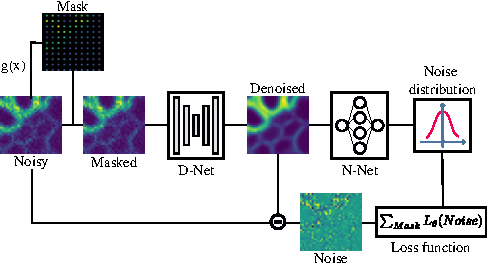
\includegraphics[width=\columnwidth]{fig_plomberie.pdf}}
\caption{Training setup.
For each mini-batch, a random grid is drawn.
The masking function $x\mapsto g(x)$ is applied on each element of the grid, replacing the original pixels in the masked image.
The denoised image predicted by the D-net is fed to the N-net that predicts a noise distribution for each pixel.
The loss function is then computed on each element of the grid.
}
\label{fig:plumbing}
\end{center}
\end{figure}

\label{sec:experiments}
\subsection{Model Architecture}
\label{sec:architectures}
\paragraph{D-net}
The function $\mu_{\theta_d}$ is parametrized by a U-net, with slight architecture modifications.
Architecture and training information can be found in Appendix\ref{si:implementation}.
The receptive field of this network is 35x35 pixels, which means that the network may use pixels from the neighborhood that are masked.
At test-time, we averaged the prediction of the image with the predictions of its transposed and flipped versions on each axis, which improves performances.

\paragraph{N-net}
In the Gaussian Mixture Model (GMM) case, the network has several outputs: for a mixture of $N$ Gaussian distributions, there are $N$ variances, $N-1$ means (the last mean is computed to ensure that the resulting distribution is centered) and $N$ mixture weights parametrized by the N-net.
In the case where $N=1$, the function $\sigma_{\theta_n}: \mathbb{R} \to \mathbb{R}$ describing the local variance of the noise distribution is a fully-connected deep neural network with several hidden layers. This choice is motivated by the large expressivity of such a network, necessary to approximate complex noise distributions. In practice, it is applied to each pixel, so it is implemented efficiently as a fully convolutional network using only 1x1 convolutional layers. The full architecture details for both models are available in Appendix\ref{si:implementation}.

%This choice is motivated by the fact that such networks can be trained in a supervised way with a clean image $X$ as input and the following cost function, where $Y$ is a corrupted observation of $X$ \textcolor{red}{il faut l'llustrer dans les supplementary non ?}:$y\mapsto\varphi_{0,\sigma_n^2}(x)$.
%The essential aspect of the architecture is that the network contain no spatial convolution (only 1x1 convolutions), otherwise the noise distribution is not well described by the network. This is consistent with our model, in which the noise is independent of the neighborhood.

\subsection{Datasets}
\label{sec:datasets}
We train and evaluate our method on 6 publicly available datasets of microscopy images. In those datasets, ground truth ($X$) is estimated by averaging several observations ($Y$) of the same field-of-view (FOV).
This allows to have access to an estimation of the noise $Y-X$, which we refer to as \textit{real noise} in this article.

The 3 first datasets (\emph{PN2V-C}, \emph{PN2V-MN}, \emph{PN2V-MA}) have been published along with the PN2V method \cite{krull2019probabilistic}, each is composed of several observations of one single FOV.
For a fair comparison, we use the same training and evaluation sets as the authors: for each sample type the whole dataset is used for training, and only a subset of the FOV is used for evaluation (see Appendix\ref{si:datasetxp} for details).
The 3 last datasets are the 3 channels of the W2S dataset \cite{zhou2020w2s} referred to as \emph{W2S-1}, \emph{W2S-2} and \emph{W2S-3}.
The dataset is composed of 120 FOV, the first 80 are used for training and the last 40 for evaluation (see Appendix\ref{si:datasetxp} for more details).
Following the authors, for each FOV, only one observation is used for training and for evaluation, which better corresponds to a real setting where only one observation per FOV is available.

\subsection{Masking procedure}
\label{sec:masking}
Following \cite{batson2019noise2self}, we mask pixels along a grid and compute the loss only on masked pixels.
We obtained the best results by replacing the central value by the weighted average of the 8 direct neighbors with Gaussian weights ($\sigma=1$).
The drawback of masking along a grid is that pixels are masked at fixed relative positions with regards to the central pixel.
If grid spacing is too small, then too many masked pixels are present in the receptive field and perturb the performances, because the available information is reduced.
On the other hand, the larger the spacing, the less pixels are used for training, which reduces dramatically training efficiency.
In order to push the limits of this trade-off, we use a random dynamic spacing between 3 and 5 pixels, which allows to have relative positions of masked pixels that change randomly.
On average, $6.8\%$ of the image is masked.

Furthermore, we observed that datasets \emph{PN2V-C} and \emph{PN2V-MA} display axial correlation in the noise, for those datasets we adapted the masking procedure introduced in \cite{broaddus2020removing}: the replacement value was computed on a neighborhood excluding the neighbors along the correlation axis, and neighbors were masked along this axis, within an extent of 3 pixels. This can be determined easily in a self-supervised setup because the neural network tends to amplify the noise correlation.

\subsection{Training}
\label{sec:training}
Networks are trained using Adam optimizer with a learning rate of $4\cdot10^{-4}$, decreased by $1/2$ on plateau of 30 epochs until $10^{-6}$. We train networks for 400 epochs of 200 steps.
Training time is about 2 min per epoch on a NVIDIA Tesla P4.
We obtain better and more reproducible results using the weights of the trained model at the last epoch instead of the weights of the model with the best validation loss, possibly because the loss is a bad proxy for the denoising performances. For that reason, we do not use a validation step.
Batch size is set to 1, and each batch is split into 100 (overlapping) tiles of 96x96 pixels.
Tiles are augmented with random horizontal and/or vertical flip and/or a random rotation with an angle chosen within $(90^\circ, 180^\circ, 270^\circ)$, except for datasets with axial noise correlation where axes transpositions are avoided.

\subsection{Evaluation}
We compared denoised image to ground truth with the classical Peak Signal-to-Noise Ratio (PSNR) metric.
However, PSNR is not highly indicative of perceived similarity, in particular it does not reflect similarity of high frequency information such as textures and local contrasts \cite{wang2004image}, that denoising methods tend to reduce. It is thus essential to have other metrics that take them into account.
To address this shortcoming, we used Structural Similarity (SSIM) that take textures and edges into account \cite{wang2004image}, computed as in the original work.

\section{Results}
\label{sec:results}
\subsection{Noise estimation}
\label{sec:results:noise}
\paragraph{Estimation on synthetic noise}
To evaluate the capacity of the N-net to capture blindly different noise distributions, we generated 3 datasets by adding synthetic noise to the ground truth of dataset \textit{W2S-1}, and we chose the parameters of the noise models so that PSNR of noisy images match the one of the original dataset (in a range of $\pm0.1$dB).
We used 3 classical noise models: additive Gaussian, Poisson-Gaussian (which is a good model for shot noise) and speckle (see Appendix\ref{si:synthetic} for details).
Empirical and predicted distributions of the noise standard deviation are illustrated in Fig.~\ref{fig:noisestd}.
One of the most striking result of this experiment is that for the 3 cases of synthetic noise, the predicted standard deviation provided by the N-net is a very sharp approximation of the known theoretical standard deviation.
It shows in particular that our method is able to capture the different noise distributions even in areas where signal is rare.
\begin{figure}[!htbp]
\vskip -0.1in
\begin{center}
\centerline{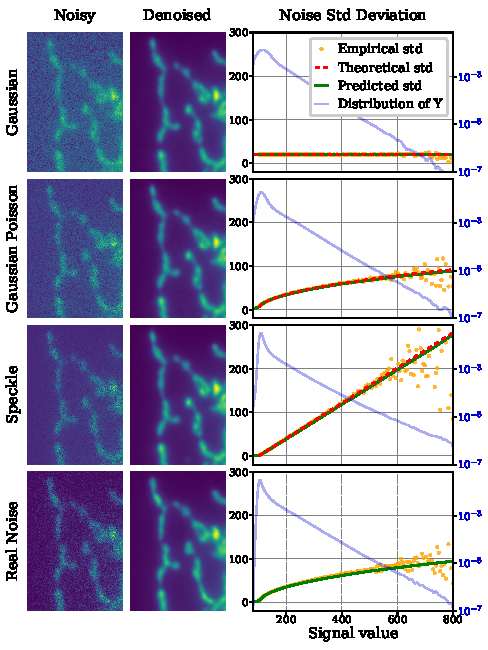
\includegraphics[width=\columnwidth]{fig_noise_std.pdf}}
\caption[Noise estimation]{Noise estimation.
For 3 models of synthetic noise as well as the real noise, the plots display the empirical standard deviation of the noise $Y - X$, as well as the predicted standard deviation of the noise by the N-net as a function of $X$ (note that display range was shrinked in Y-axis for visualization purposes.).
Theoretical standard deviation of the noise is displayed for the 3 models of synthetic noise.
The empirical distribution of $Y$ is displayed in blue, in logarithmic scale.
Examples of noisy images corrupted with the corresponding noise model and the predicted denoised images are displayed above each graph.}
\label{fig:noisestd}
\end{center}
\end{figure}


\paragraph{Improving estimation on real noise}
\label{sec:exp:real:noise}
We observed that contrary to the classical noise models considered in the denoising literature, real noise often displays a certain amount of skewness, as illustrated in Fig.~\ref{fig:skewness}.
In order to be able to capture this aspect, we predict a Gaussian mixture model (GMM) instead of a simple Gaussian model as described in Section~\ref{sec:model}. Fig.~\ref{fig:skewness} shows that noise skewness is well described by the predicted model, and the noise distribution is better described by a GMM than by a single Gaussian.
This applies for all datasets and the equivalent figures can be found in Appendix\ref{si:skewness}.
In this example, it is interesting to note that the Kullback–Leibler divergence between the empirical noise distribution and the predicted distribution (as a function of the signal value) is improved by considering a GMM instead of a unimodal distribution.
This supports the use of our flexible N-net to capture a large variety of noise distributions (with multimodality and/or skewness) which can be observed in experimental datasets.
This comment paves the way to several perspectives for our work such as the design of statistically consistent model selection procedures to choose automatically the number of mixing components.
Such approaches have been proposed in more simple cases using for instance penalized maximum likelihood based algorithms.
This remains an open problem in our framework and we leave this topic for future research.
\begin{figure}[!htbp]
\vskip -0.1in
\begin{center}
\centerline{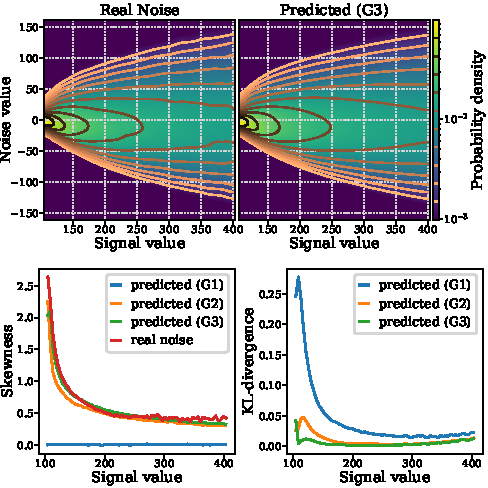
\includegraphics[width=\columnwidth]{fig_skewness_w2s-1.pdf}}
\caption{Real noise estimation for dataset \textit{W2S-1}.
The two left graphs represent the empirical distribution of the noise $Y - X$ as a function of $X$ and the corresponding predicted noise distribution for a 3-component-GMM.
The probability density is normalized for each signal value bin.
Skewness of real and predicted noise distribution as a function of $X$, estimated with Pearson's moment coefficient of skewness.
Kullback–Leibler divergence between real noise distribution and predicted distribution generated by each model, as a function of $X$.
\textit{G1} stands for Gaussian model, \textit{G2} for a 2-component-GMM and \textit{G3} a 3-component-GMM.
}
\label{fig:skewness}
\end{center}
\end{figure}

\subsection{Denoising performances}
\label{sec:perf}
\begin{table*}[!htbp]
\vskip -0.15in
\caption{Evaluation of our method on 6 datasets with PSNR/SSIM metrics.
SSIM estimates structural similarity (sharpness).
Metrics computed on noisy images are displayed in the \textit{Noisy} column.
The supervised version of our method was not trained for PN2V datasets as they cannot be split into independent train/evaluation sets.
For DecoNoising and N2V, PSNR are taken from \cite{goncharova2020} and SSIM are computed on prediction made by networks we trained (see section~\ref{si:baselines}).
\textit{Gaussian} corresponds to the optimal Gaussian baseline defined in section~\ref{sec:perf}.
\textit{Neigh2Neigh} stands for Neighbor2Neighbor.
Results for our method predicting a Gaussian model are shown in column \textit{Ours (G1)} (see Appendix~Table~\ref{si:table:results} for 2/3-component GMM).
Best PSNR $\pm0.1dB$ / SSIM $\pm1\permille$ scores are underlined.}
\label{table:results}
\begin{center}
\begin{small}
\begin{sc}
\resizebox{\textwidth}{!}{
\begin{tabular}{lcccccc}
\toprule
Method/Dataset & PN2V-C & PN2V-MN & PN2V-MA & W2S-1 & W2S-2 & W2S-3 \\
\midrule
Noisy & $28.98$ / $0.7713$ & $28.10$ / $0.6836$ & $23.71$ / $0.3731$ & $21.85$ / $0.3490$ & $19.33$ / $0.2256$ & $20.39$ / $0.2232$ \\
Gaussian & $34.92$ / $0.9409$ & $35.53$ / $0.9392$ & $34.07$ / $0.8739$ & $33.87$ / $0.9326$ & $32.27$ / $0.8531$ & $34.66$ / $0.9013$\\
Supervised & $NA$ / $NA$ & $NA$ / $NA$ & $NA$ / $NA$ & $35.22$ / $0.9608$ & $33.24$ / $0.8828$ & $36.31$ / $0.9252$\\
N2V & $35.85$ / $0.9404$ & $35.86$ / $0.9419$ & $33.35$ / $0.8384$ & $34.30$ / $0.9026$ & $31.80$ / $0.8311$ & $34.65$ / $0.8637$\\
DecoNoising & $36.39$ / $0.9483$ & $36.34$ / $0.9489$ & $34.04$ / $0.8633$ & $34.90$ / $0.9169$ & $32.31$ / $0.8524$ & $35.09$ / $0.9051$\\
Neigh2Neigh & $34.42$ / $0.9519$ & $34.01$ / $0.9070$ & $32.70$ / $0.8521$ & $34.74$ / $0.9552$ & $32.96$ / $0.8739$ & $36.14$ / $0.9216$\\
FBI-Denoiser & $36.23$ / $0.9556$ & $36.85$ / $0.9609$ & $32.89$ / $0.8344$ & $34.40$ / $0.9500$ & $32.26$ / $0.8452$ & $34.94$ / $0.8910$\\
Ours (G1) & $\underline{38.33}$ / $\underline{0.9754}$ & $\underline{39.08}$ / $\underline{0.9776}$ & $\underline{34.79}$ / $\underline{0.8905}$ & $\underline{35.33}$ / $\underline{0.9619}$ & $\underline{33.46}$ / $\underline{0.8867}$ & $\underline{36.57}$ / $\underline{0.9263}$\\

\bottomrule
\end{tabular}
}
\end{sc}
\end{small}
\end{center}
\vskip -0.1in
\end{table*}

We compared our method to 6 baselines: D-net trained in a supervised setup with L2 objective (with all other training and prediction hyperparameters unchanged), N2V, DecoNoising, which is the self-supervised blind denoising method that has shown best results on the datasets we considered, Neighbor2Neighbor and FBI-Denoiser, as well as one of the most simple denoising method: convolution by a Gaussian, whose standard deviation is chosen to maximize the PSNR on the evaluation dataset.
We believe the latter makes a good reference, as it is one of the simplest denoising methods, and it removes noise efficiently but also other high-frequency information such as local contrasts. Training procedure is detailed in Appendix\ref{si:baselines}.

The considered metrics are summarized in Table~\ref{table:results}.
Our method significantly outperforms the baselines both in terms of PSNR and SSIM on all datasets.
Note that datasets PN2V-C and PN2V-MA have horizontally-correlated noise (that we take into account: see Section~\ref{sec:datasets}), which significantly lowers the performances of methods that are sensitive to it, such as FBI-Denoiser or N2V.
For the version predicting a simple Gaussian distribution, the average PSNR gain over DecoNoisng is $+1.42$dB.
This is also confirmed by the visual aspect, displayed in Fig.~\ref{fig:images}: our method produces images closer to the ground truth, smoother, sharper, more detailed and without visual artifacts.
Remarkably, our method performs significantly better than the supervised method CARE \cite{weigert2017content}, with an average PSNR gain of $+1.49$dB (compared to PSNR values reported in \cite{goncharova2020}).
Moreover, our method also performs better than its supervised counterpart with an average gain of $+0.21$dB (see Table~\ref{table:results}).
This could be explained by the fact that training with masking induces a lower dependency to central pixel compared to supervised training, and thus pushes the network to make better use of the neighborhood.

\begin{figure*}[!hbp]
% \vskip -0.1in
\includegraphics[width=\textwidth]{fig_images.pdf}
\caption{Visual comparison of denoising on the considered datasets. For each dataset a $256$x$256$ portion of an evaluation image is displayed, on which metrics are computed and displayed below. Training of baselines is described in section~\ref{si:baselines}. \textit{Gaussian} corresponds to the optimal Gaussian baseline defined in section~\ref{sec:perf}.}
\label{fig:images}
\end{figure*}

\subsection{Ablation experiments}

To better understand the contribution of the N-net and other hyperparameters, we ran ablation experiments in Table~\ref{table:ablation}. The N-net has a very significant impact on performances, in particular when training is short (e.g. as in N2V, N2S \cite{krull2018noise2void, goncharova2020}). We observe that the N-net greatly stabilizes the training\footnote{As an illustration of the excellent training stability, we measured a SEM of $6\cdot10^{-3}$ for the PSNR on dataset W2S-1 over 5 runs.} and improves convergence speed (see Fig. ~\ref{si:fig:convergence}). We also observe that in all our hyperparameter settings that adding the N-net always improves performances over L2 objective, although not always significantly.

From the perspective of our framework, the L2 objective (as used in N2V, N2S) can be understood as a particular case of the N-net predicting a constant unit Gaussian noise. When the actual noise is significantly different from it, the N-net has a stronger impact (e.g. \textit{Speckle} in Fig. ~\ref{si:fig:convergence}B).
From a statistical perspective, it is known that considering a sufficiently rich noise model is crucial in deconvolution problem for signal estimation (misspecifying the noise density can lead to very poor deconvolution estimators for instance). This was a motivation to introduce the N-net.
It is worth noting that considering mixture models improves the PSNR in two datasets out of six (Table~\ref{si:table:results}).
As mentioned in Section~\ref{sec:results:noise}-b) an optimal and data-driven choice of the number of components remains an open (and challenging) statistical problem but we believe that such experiments support future research in this direction.

\begin{table}[ht]
\caption{Ablation experiment on dataset W2S-1.
\textit{N2V}: Noise2Void (L2).
+ \textit{N-net (G1)}: N-net with a single Gaussian component.
+ \textit{LT}: Longer training, see ~\ref{sec:training}.
\textit{Ours} as described in ~\ref{sec:experiments}.
}
\label{table:ablation}
\begin{center}
\begin{small}
\begin{sc}
\begin{tabular}{lcc}
\toprule
Condition & PSNR & SSIM \\
\midrule
N2V & $34.30$ & $0.9026$\\
 + N-net (G1) & $34.99$ & $0.9572$\\
 + N-net (G1) + LT & $35.22$ & $0.9608$\\
Ours with N-net (G1)& $\underline{35.33}$ & $\underline{0.9619}$\\
\bottomrule
\end{tabular}
\end{sc}
\end{small}
\end{center}
\end{table}

\section{Discussion and Limitations}
\label{sec:discussion}
We introduced a novel self-supervised blind-denoising method modeling both the signal and the noise distributions. We believe its simplicity, performances and the interpretability of the noise distribution will be useful both in practical applications, and as a basis for future research.

First, future works could consider more complex families of noise distributions such as structured or non-centered noises, that can also arise in real-life setups. In particular, \cite{lehtinen2018noise2noise} managed to remove very structured non-centered noises such as overlaid text. With stronger assumptions and architecture changes, it might be possible to capture such noises.

Second, more theoretical works could explore the model proposed in this work  (i) to obtain identifiability of model \eqref{eq:def:Y} and extend \cite{gassiat:lecorff:lehericy:2021} to state-dependent standard deviations and (ii) to establish rates of convergence for the proposed estimators.

Finally, it would also be interesting to understand the role of the central pixel at test time, as it has a significative impact on performance: it depends on the masking procedure and the convolutional architecture, but the network is not trained explicitly to use it. Our mathematical modeling could be a good basis to study this specific dependency on the central pixel.





% An example of a floating figure using the graphicx package.
% Note that \label must occur AFTER (or within) \caption.
% For figures, \caption should occur after the \includegraphics.
% Note that IEEEtran v1.7 and later has special internal code that
% is designed to preserve the operation of \label within \caption
% even when the captionsoff option is in effect. However, because
% of issues like this, it may be the safest practice to put all your
% \label just after \caption rather than within \caption{}.
%
% Reminder: the "draftcls" or "draftclsnofoot", not "draft", class
% option should be used if it is desired that the figures are to be
% displayed while in draft mode.
%
%\begin{figure}[!t]
%\centering
%\includegraphics[width=2.5in]{myfigure}
% where an .eps filename suffix will be assumed under latex,
% and a .pdf suffix will be assumed for pdflatex; or what has been declared
% via \DeclareGraphicsExtensions.
%\caption{Simulation results for the network.}
%\label{fig_sim}
%\end{figure}

% Note that the IEEE typically puts floats only at the top, even when this
% results in a large percentage of a column being occupied by floats.


% An example of a double column floating figure using two subfigures.
% (The subfig.sty package must be loaded for this to work.)
% The subfigure \label commands are set within each subfloat command,
% and the \label for the overall figure must come after \caption.
% \hfil is used as a separator to get equal spacing.
% Watch out that the combined width of all the subfigures on a
% line do not exceed the text width or a line break will occur.
%
%\begin{figure*}[!t]
%\centering
%\subfloat[Case I]{\includegraphics[width=2.5in]{box}%
%\label{fig_first_case}}
%\hfil
%\subfloat[Case II]{\includegraphics[width=2.5in]{box}%
%\label{fig_second_case}}
%\caption{Simulation results for the network.}
%\label{fig_sim}
%\end{figure*}
%
% Note that often IEEE papers with subfigures do not employ subfigure
% captions (using the optional argument to \subfloat[]), but instead will
% reference/describe all of them (a), (b), etc., within the main caption.
% Be aware that for subfig.sty to generate the (a), (b), etc., subfigure
% labels, the optional argument to \subfloat must be present. If a
% subcaption is not desired, just leave its contents blank,
% e.g., \subfloat[].


% An example of a floating table. Note that, for IEEE style tables, the
% \caption command should come BEFORE the table and, given that table
% captions serve much like titles, are usually capitalized except for words
% such as a, an, and, as, at, but, by, for, in, nor, of, on, or, the, to
% and up, which are usually not capitalized unless they are the first or
% last word of the caption. Table text will default to \footnotesize as
% the IEEE normally uses this smaller font for tables.
% The \label must come after \caption as always.
%
%\begin{table}[!t]
%% increase table row spacing, adjust to taste
%\renewcommand{\arraystretch}{1.3}
% if using array.sty, it might be a good idea to tweak the value of
% \extrarowheight as needed to properly center the text within the cells
%\caption{An Example of a Table}
%\label{table_example}
%\centering
%% Some packages, such as MDW tools, offer better commands for making tables
%% than the plain LaTeX2e tabular which is used here.
%\begin{tabular}{|c||c|}
%\hline
%One & Two\\
%\hline
%Three & Four\\
%\hline
%\end{tabular}
%\end{table}


% Note that the IEEE does not put floats in the very first column
% - or typically anywhere on the first page for that matter. Also,
% in-text middle ("here") positioning is typically not used, but it
% is allowed and encouraged for Computer Society conferences (but
% not Computer Society journals). Most IEEE journals/conferences use
% top floats exclusively.
% Note that, LaTeX2e, unlike IEEE journals/conferences, places
% footnotes above bottom floats. This can be corrected via the
% \fnbelowfloat command of the stfloats package.








% if have a single appendix:
%\appendix[Proof of the Zonklar Equations]
% or
%\appendix  % for no appendix heading
% do not use \section anymore after \appendix, only \section*
% is possibly needed

% use appendices with more than one appendix
% then use \section to start each appendix
% you must declare a \section before using any
% \subsection or using \label (\appendices by itself
% starts a section numbered zero.)
%


\appendices

%\renewcommand{\thetable}{A\arabic{table}}
%\renewcommand{\thefigure}{A\arabic{figure}}
%\setcounter{table}{0}
%\setcounter{figure}{0}


\subsection{Additional Implementation details}
\label{si:implementation}
\subsubsection{Networks and training}
\paragraph{D-net architecture details}
The architecture is based on U-net \cite{ronneberger2015u}.
We propose several changes from the original version: we do not crop the image and use zero-padding instead, we use 2 levels of contractions/expansions with 64 filters, expansions are performed by an upsampling layer with nearest-neighbor approximation directly followed by 2x2 convolution.
We also add two layers of 1x1 convolution with 64 filters and ReLU activation at the end of the network, and set no activation function at the output layer.

\paragraph{N-net architecture details}
In the case of a Gaussian noise, the N-net is composed 3 successive blocks, each block being composed of two 1x1 convolutions layers of 64 filters, each followed by a non-linear activation layer (alternatively tanh and leaky ReLU with alpha parameter set to $0.1$). A convolution 1x1 with a single channel followed by an exponential activation function is placed after the last block (to ensure that the predicted $\sigma$ is positive).

In the case where the N-net predicts a GMM with N components with weights $(\alpha_{k,\theta_n})_{1\leqslant k\leqslant N}$, means $(\mu_k)_{1\leqslant k\leqslant N}$ and variances $(\sigma^2_{k,\theta_n})_{1\leqslant k\leqslant N}$, the second block is connected to three distinct blocks, each connected to a convolution 1x1 with:
\begin{itemize}
  \item N channels, followed by an exponential activation function to predict $\sigma_{k,\theta_n}$.
  \item N channels, followed by a softmax activation to predict $\alpha_{k,\theta_n}.$\footnote{When $N=2$, only one channel is used and followed by a sigmoid activation function.}
  \item N-1 channels to predict the distribution means $\mu_{k,\theta_n}$.
\end{itemize}
To ensure that the distribution is centered, the center of the last distribution is computed as
$$
\mu_{N,\theta_n} = - \frac{1}{\alpha_{N,\theta_n}} \sum_{k=1}^{N-1}\alpha_{k,\theta_n}\cdot\mu_{k,\theta_n}\,.
$$

\subsection{Baselines}
\label{si:baselines}
\begin{itemize}
  \item DecoNoisng was trained using the source code provided by the authors, using no positivity constraint: \url{https://github.com/juglab/DecoNoising}. For N2V we used the same code without the convolution.
  \item FBI-Denoiser was trained using the code provided by authors: \url{https://github.com/csm9493/FBI-Denoiser/tree/de86420934a2416d4052dfa1298334af0d2ca49f}. We used same training options as for FMD datasets that are also fluorescence microscopy datasets. We tried to double the number of epochs without improvement.
  \item Neighbor2Neighbor was trained using the code provided by the authors: \url{https://github.com/TaoHuang2018/Neighbor2Neighbor/tree/e66389ebef1e64d306d8fcb95f096cf427243452}. As this method was not trained on fluorescence microscopy datasets, we tried to optimise hyperparameters as best as we could on dataset W2S-1 and used the same hyperparameters for all datasets. More precisely we tested $\gamma=1$ and $\gamma=2$, an initial learning rate of $3\cdot10^{-4}$ or $1\cdot10^{-4}$ as suggested by the authors. Moreover, we also increased the number of epochs from 100 to 1000, and tried to decrease the learning rate to $1\cdot10^{-6}$ instead of $2\cdot10^{-5}$ (which surprisingly led to much lower performances). In the end, we used $\gamma=1$, an initial learning rate of $3\cdot10^{-4}$, a minimal learning rate of $2\cdot10^{-5}$ and 1000 epochs.
\end{itemize}

\subsection{Datasets}
\subsubsection{Experimental Datasets}
\label{si:datasetxp}
\paragraph{Datasets published along with the PN2V \cite{krull2019probabilistic}}
\begin{itemize}
  \item \emph{Convallaria} dataset, referred to as \emph{PN2V-C} is composed of 100 images of size $1024$x$1024$. Evaluation subset is: $Y\in\interval{0}{512}, X\in\interval{0}{512}$.
  \item \emph{Mouse skull nuclei} referred to as \emph{PN2V-MN} is composed 200 images of size $512$x$512$. Evaluation subset is: $Y\in\interval{0}{512}, X\in\interval{0}{256}$.
  \item \emph{Mouse Actin} referred to as \emph{PN2V-MA} is composed of 100 images of size $1024$x$1024$. Evaluation subset is: $Y\in\interval{0}{1024}, X\in\interval{0}{512}$.
\end{itemize}

The \emph{PN2V-C} and \emph{PN2V-MA} datasets are acquired on a spinning disc confocal microscope and \emph{PN2V-MN} dataset is acquired with a point scanning confocal microscope.
Datasets can be respectively downloaded at: \url{https://doi.org/10.5281/zenodo.5156913}, \url{https://doi.org/10.5281/zenodo.5156960} and \url{https://doi.org/10.5281/zenodo.5156937}

We observed that datasets acquired with a spinning disc confocal microscope display axial noise correlation (see \ref{sec:datasets}).

\paragraph{Datasets published in \cite{zhou2020w2s}}

We used the 16-bit raw images kindly provided by the authors.
The dataset is composed of 120 FOV of 400 observations of size $512$x$512$ pixels.
The first 80 are used for training and the last 40 for evaluation.
Following the authors, for each FOV, only the observation of index 249 is used for training and evaluation
images are acquired with a electron-multiplying charge-coupled device camera on a wide-field microscope.
It can be downloaded at: \url{https://datasets.epfl.ch/w2s/W2S_raw.zip}

\paragraph{Normalization}

Images were normalized using the modal value as center and the difference between modal value and $95\%$ percentile as scale factor, computed on the whole dataset.
This is relevant in fluorescence microscopy data where signal is often less abundant than background with proportion that vary among images and signal distribution often has a heavy tail towards high values.

\paragraph{Metrics}
For the 6 chosen datasets, images are encoded in 16-bit.
PSNR is defined as $PSNR = 10 \log_{10}(d/\mathrm{MSE})$, with $d$ the maximum possible pixel value range of the image and $\mathrm{MSE}$ the mean squared error.
For 8-bit encoded images d is simply $255$, and for 16-bit images it would be $65635$ but this does not correspond to the actual possible range of microscopy data, thus the actual range of values of each ground truth image is used. This is also what is done in \cite{goncharova2020} as we obtain the same PSNR values for raw images.
The same applies for SSIM computation.

\subsubsection{Synthetic noise datasets}
\label{si:synthetic}
\begin{itemize}
  \item Additive Gaussian: $Y = X + \varepsilon$ with $\varepsilon \sim \mathcal{N}(0, \sigma^2)$, $\sigma=20$.
  \item Poisson-Gaussian: $Y = X + (\alpha * (X-\underline{X}) + \eta^2 )^{1/2}\varepsilon$  with $\varepsilon \sim \mathcal{N}(0, 1)$, $\alpha=5, \eta=12$ and $\underline{X}$ being the minimal value of the ground truth on the whole dataset.
  \item Speckle: $X = X + (X-\underline{X})\varepsilon$  with $\varepsilon \sim \mathcal{N}(0, \sigma^2)$, $\sigma=0.405$ and $\underline{X}$ being the minimal value of the ground truth on the whole dataset.
\end{itemize}

% \subsection{Results on additional datasets}
% In table~\ref{si:table:datasetsup} we report performance on additional datasets, including a natural image dataset, and comparison with other methods.
% FMD datasets \cite{zhang2019poisson} are composed of fluorescence microscopy images. Same training and evaluation set as the original article are used.
% BSD68 \cite{martin2001database} is a natural image dataset; for this dataset, the training and validation set of BSD500 \cite{arbelaez2010contour} (400 images in total) is used for training. Images were corrupted with AWGN with $\sigma=25$.
% All the datasets used in this table are composed of 8-bit images, thus the range used for metric computation is set to 255.

% \begin{table*}[ht]
% \caption{Evaluation of the performances on additional datasets with PSNR/SSIM metrics. Metric for FBI-Denoiser are reported from \cite{byun2021fbi}, note that this method is not completely blind as it assumes a Gaussian-Poisson noise. Metrics for Laine et al. are reported from \cite{laine2019high}, note that this method is not blind as it requires the noise model. Metrics for Self2Self are reported from \cite{quan2020self2self}. Best PSNR $\pm0.1dB$ / SSIM $\pm1\permille$ scores are underlined.}
% \label{si:table:datasetsup}
% \begin{center}
% \begin{sc}
% \begin{tabular}{lcccccc}
% \toprule
% Dataset & Noisy & Ours (G1) & N2V & FBI-Denoiser & Laine et al. & Self2Self \\
% \midrule
% FMD Confocal-Fish & $22.81$ / $0.4416$ & $\underline{32.56}$ / $0.8822$ & $31.92$ / $0.8831$ & $32.22$ / $\underline{0.8853}$ & $NA$ / $NA$ & $NA$ / $NA$ \\
% FMD Confocal-Mice & $29.38$ / $0.6657$ & $\underline{38.48}$ / $\underline{0.9655}$ & $37.54$ / $0.9611$ & $38.32$ / $0.9637$ & $NA$ / $NA$ & $NA$ / $NA$ \\
% BSD68 (G25) & $20.17$ / $0.3819$ & $\underline{28.92}$ / $\underline{0.8217}$ & $27.72$ / $0.794$ & $NA$ / $NA$ & $\underline{28.84}$ / $0.814$ & $28.70$ / $0.803$ \\
% \bottomrule
% \end{tabular}
% \end{sc}
% \end{center}
% \end{table*}

\subsection{Impact of the N-net}
\label{si:impactnnet}
\begin{figure}[ht]
\begin{center}
\centerline{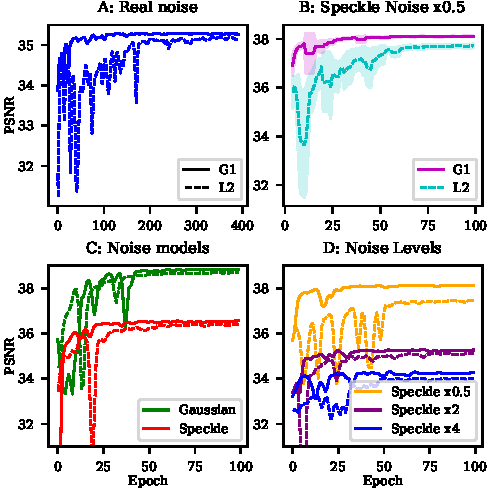
\includegraphics[width=\columnwidth]{fig_convergence.pdf}}
\caption{PSNR at each epoch on the test set for N-net (G1) or D-net only (L2). A: training on real noise. B, C: training on different models/levels of synthetic noise added to ground truth image. B: \textit{Gaussian} and \textit{Speckle} correspond to noises presented in 5.1, that have no and high signal dependency respectively. C: \textit{Speckle} with variance multiplied by 0.5, 2 and 4. D: Mean and SEM over 5 runs.}
\label{si:fig:convergence}
\end{center}
\end{figure}

\begin{table*}[ht]
\caption{Evaluation of the impact of N-net on performances with PSNR/SSIM metrics. Comparison between our method predicting a GMM with 1, 2, or 3 components (respectively G1, G2, G3) and D-net only trained with L2 loss (with training and prediction scheme unchanged).
Best PSNR $\pm0.1dB$ / SSIM $\pm1\permille$ scores are underlined.}
\label{si:table:results}
\begin{center}
\begin{sc}
\begin{tabular}{lccccc}
\toprule
Dataset & Noisy & Ours (G1) & Ours (G2) & Ours (G3) \\
\midrule
PN2V-C & $28.98$ / $0.7713$ & $38.33$ / $\underline{0.9754}$ & $\underline{38.47}$ / $0.9738$ & $38.28$ / $\underline{0.9756}$ \\
PN2V-MN & $28.10$ / $0.6836$ & $39.08$ / $\underline{0.9776}$ & $\underline{39.22}$ / $\underline{0.9779}$ & $\underline{39.18}$ / $\underline{0.9780}$ \\
PN2V-MA & $23.71$ / $0.3731$ & $\underline{34.79}$ / $\underline{0.8905}$ & $34.68$ / $0.8880$ & $\underline{34.70}$ / $0.8877$ \\
W2S-1 & $21.85$ / $0.3490$ & $\underline{35.33}$ / $\underline{0.9619}$ & $\underline{35.27}$ / $\underline{0.9623}$ & $\underline{35.27}$ / $\underline{0.9624}$ \\
W2S-2 & $19.33$ / $0.2256$ & $\underline{33.46}$ / $\underline{0.8867}$ & $\underline{33.48}$ / $\underline{0.8871}$ & $\underline{33.47}$ / $\underline{0.8871}$ \\
W2S-3 & $20.39$ / $0.2232$ & $\underline{36.57}$ / $\underline{0.9263}$ & $\underline{36.60}$ / $\underline{0.9269}$ & $\underline{36.59}$ / $\underline{0.9269}$ \\
\bottomrule
\end{tabular}
\end{sc}
\end{center}
\end{table*}
%\FloatBarrier

%\FloatBarrier
\subsection{Noise estimation}
\label{si:skewness}
This section contains the figures corresponding to Fig~\ref{fig:skewness} for each dataset.
Note that they are computed using regular signal value bins and excluding signal values greater to the $99.5\%$ percentile of the dataset so that there are enough observed samples in each bin to compute statistically significant metrics.

\begin{figure}[ht]
\begin{center}
\centerline{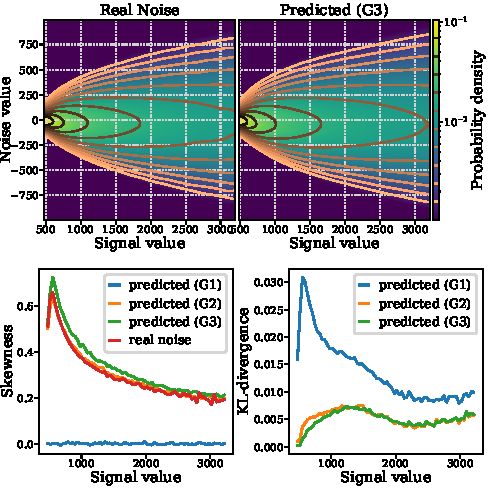
\includegraphics[width=\columnwidth]{fig_skewness_pn2v-C.pdf}}
\caption{Real noise estimation for dataset \textit{PN2V-C}. See main text Fig~\ref{fig:skewness}.
}
\end{center}
\end{figure}

\begin{figure}[ht]
\begin{center}
\centerline{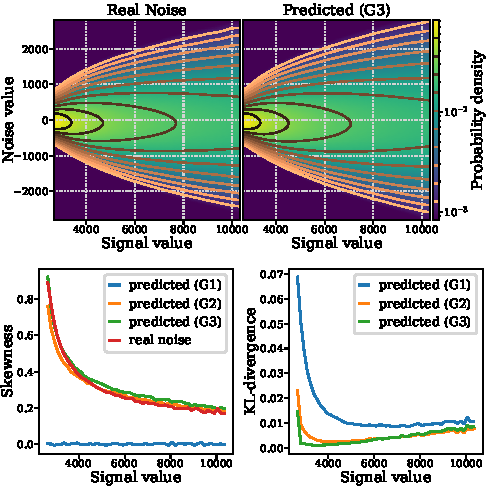
\includegraphics[width=\columnwidth]{fig_skewness_pn2v-MN.pdf}}
\caption{Real noise estimation for dataset \textit{PN2V-MN}. See main text Fig~\ref{fig:skewness}.
}
\end{center}
\end{figure}

\begin{figure}[ht]
\begin{center}
\centerline{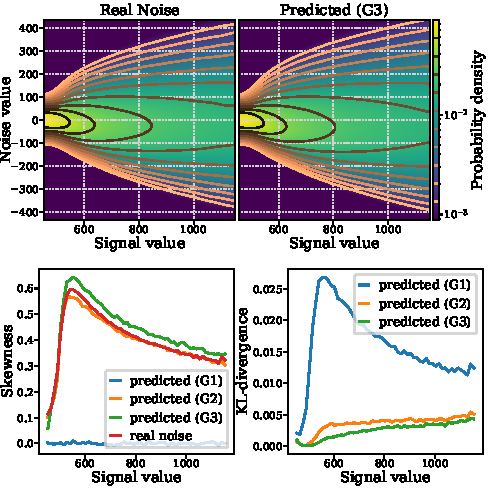
\includegraphics[width=\columnwidth]{fig_skewness_pn2v-MA.pdf}}
\caption{Real noise estimation for dataset \textit{PN2V-MA}. See main text Fig~\ref{fig:skewness}.
}
\end{center}
\end{figure}

\begin{figure}[ht]
\begin{center}
\centerline{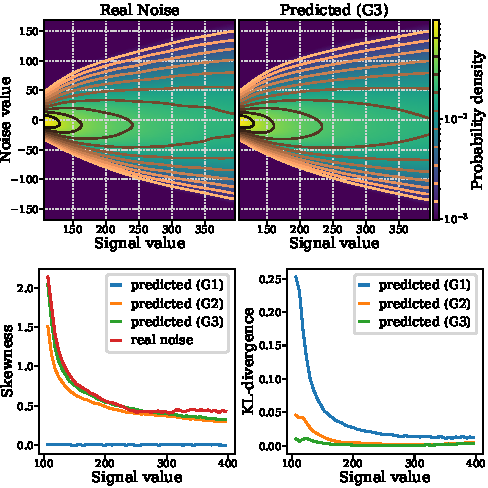
\includegraphics[width=\columnwidth]{fig_skewness_w2s-2.pdf}}
\caption{Real noise estimation for dataset \textit{W2S-2}. See main text Fig~\ref{fig:skewness}.
}
\end{center}
\end{figure}

\begin{figure}[ht]
\begin{center}
\centerline{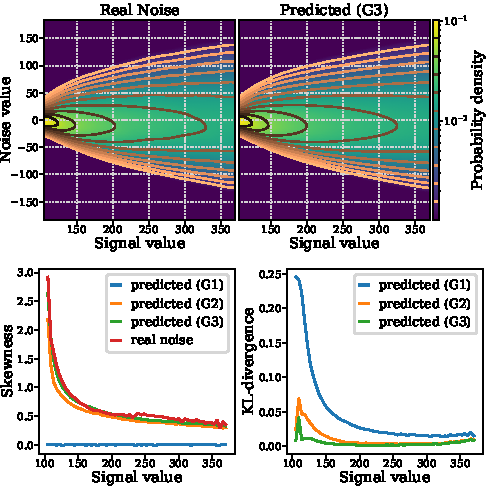
\includegraphics[width=\columnwidth]{fig_skewness_w2s-3.pdf}}
\caption{Real noise estimation for dataset \textit{W2S-3}. See main text Fig~\ref{fig:skewness}.
}
\end{center}
\end{figure}
%\FloatBarrier
\subsection{Code}
\label{sec:code}
Source code can be found at this url: \url{https://github.com/code-ssbd/ieee}.
A ready-to-use google colab notebook that includes training and evaluation procedures can be found at this address: \url{https://gist.github.com/code-ssbd/476fc09cc4efcbb834c482f0714a9d69} by clicking on the \textit{open in colab} banner. It can be executed directly through Google Colab, which only requires a Google account.


% use section* for acknowledgment
%\section*{Acknowledgment}
%
%
%The authors would like to thank...


% Can use something like this to put references on a page
% by themselves when using endfloat and the captionsoff option.
% \ifCLASSOPTIONcaptionsoff
%   \newpage
% \fi
\newpage


% trigger a \newpage just before the given reference
% number - used to balance the columns on the last page
% adjust value as needed - may need to be readjusted if
% the document is modified later
%\IEEEtriggeratref{8}
% The "triggered" command can be changed if desired:
%\IEEEtriggercmd{\enlargethispage{-5in}}

% references section

% can use a bibliography generated by BibTeX as a .bbl file
% BibTeX documentation can be easily obtained at:
% http://mirror.ctan.org/biblio/bibtex/contrib/doc/
% The IEEEtran BibTeX style support page is at:
% http://www.michaelshell.org/tex/ieeetran/bibtex/
\bibliographystyle{IEEEtran}
% argument is your BibTeX string definitions and bibliography database(s)
\bibliography{blind_denoising}
%
% <OR> manually copy in the resultant .bbl file
% set second argument of \begin to the number of references
% (used to reserve space for the reference number labels box)
%\begin{thebibliography}{1}
%
%\bibitem{IEEEhowto:kopka}
%H.~Kopka and P.~W. Daly, \emph{A Guide to \LaTeX}, 3rd~ed.\hskip 1em plus
%  0.5em minus 0.4em\relax Harlow, England: Addison-Wesley, 1999.
%
%\end{thebibliography}

% biography section
%
% If you have an EPS/PDF photo (graphicx package needed) extra braces are
% needed around the contents of the optional argument to biography to prevent
% the LaTeX parser from getting confused when it sees the complicated
% \includegraphics command within an optional argument. (You could create
% your own custom macro containing the \includegraphics command to make things
% simpler here.)
%\begin{IEEEbiography}[{\includegraphics[width=1in,height=1.25in,clip,keepaspectratio]{mshell}}]{Michael Shell}
% or if you just want to reserve a space for a photo:

%\begin{IEEEbiography}{Michael Shell}
%Biography text here.
%\end{IEEEbiography}

% if you will not have a photo at all:
%\begin{IEEEbiographynophoto}{John Doe}
%Biography text here.
%\end{IEEEbiographynophoto}

% insert where needed to balance the two columns on the last page with
% biographies
%\newpage

%\begin{IEEEbiographynophoto}{Jane Doe}
%Biography text here.
%\end{IEEEbiographynophoto}

% You can push biographies down or up by placing
% a \vfill before or after them. The appropriate
% use of \vfill depends on what kind of text is
% on the last page and whether or not the columns
% are being equalized.

%\vfill

% Can be used to pull up biographies so that the bottom of the last one
% is flush with the other column.
%\enlargethispage{-5in}



% that's all folks
\end{document}
